\documentclass[
%reprint,
%superscriptaddress,
%groupedaddress,
%unsortedaddress,
%runinaddress,
%frontmatterverbose, 
%preprint,
%showpacs,preprintnumbers,
%nofootinbib,
%nobibnotes,
%bibnotes,
amsmath,amssymb,
aps,
%twocolumn,
%pra,
prb,
%rmp,
%prstab,
%prstper,
%floatfix,
]{revtex4}

\usepackage{graphicx}% Include figure files
\usepackage{dcolumn}% Align table columns on decimal point
\usepackage{bm}% bold math

\begin{document}

\begin{flushright}
 { {\bf Author:} Burak Himmetoglu}
\end{flushright}


\begin{center}
 {\bf Details on the transport code implementation}
\end{center}
%

Scattering rates:

\begin{eqnarray}
\tau_{n {\bf k}}^{-1} &=& \frac{2 \pi}{\hbar}\, \sum_{{\bf q} \nu, m}\, \vert g_{{\bf q} \nu} \vert^2\, 
  \left( 1 - {\hat v}_{n {\bf k}} \cdot {\hat v}_{m {\bf k+q}} \right)\, 
  \Bigg\{ (n_{{\bf q}\, \nu} + f_{m, {\bf k+q}})\, \delta( \epsilon_{m, {\bf k+q}} - \epsilon_{n {\bf k}} - \hbar\omega_{L \nu} ) \nonumber\\
%
 && \qquad\qquad\qquad\qquad\qquad\qquad\qquad\qquad
   +  (1 + n_{{\bf q}\, \nu} - f_{m, {\bf k+q}})\, \delta(\epsilon_{m, {\bf k+q}} - \epsilon_{n {\bf k}} + \hbar\omega_{L \nu} )
  \Bigg\} \label{eqn:tau}
\end{eqnarray}
% 
where 

%
\begin{equation}
g_{{\bf q}\, \nu} = i\frac{e^2}{\epsilon_0\, V}\, \sum_{\bf G}\, \sum_{\alpha, \beta, s, \nu}\,
  \left( \frac{\hbar}{2\, M_s\, \omega_{{\bf q}\, \nu}} \right)^{1/2}\, 
  \frac{ (q+G)_{\alpha}\, Z^{*\, \alpha \beta}_s } {({\bf q+G}) \cdot {\bf \epsilon}_{\infty} \cdot ({\bf q+G}) }\,
  e_{s\, \beta}({\bf q} ; \nu) \label{eqn:gnu}
\end{equation}
%
Or, in a simplified approximate form 
%
\begin{equation}
\left\vert g_{{\bf q}\, \nu} \right\vert^2 = \frac{1}{q^2}\, 
  \left( \frac{e^2\, \hbar\, \omega_{L\nu}}{2 \epsilon_0\, V_{\rm cell}\, \epsilon_{\infty}} \right)\,
  \frac{\prod_{j=1}^{N} \left(1-\frac{\omega_{T j}^2}{\omega_{L \nu}^2}\right)}
       {\prod_{j \neq \nu} \left( 1 - \frac{\omega_{L j}^2}{\omega_{L \nu}^2} \right)}
\label{eqn:gnu2}
\end{equation}
%
In Eq.(\ref{eqn:tau}) the delta-function is replaced by a Gaussian smearing with adaptive smearing width:
%
\begin{eqnarray}
&& \delta(F_{n{\bf k}, \, m{\bf k+q}}) = \frac{1}{\sqrt{\pi}\, \sigma}\, 
       \exp\left[ - \frac{ F_{n{\bf k}, \, m{\bf k+q}}^2 }{\sigma^2}  \right] \nonumber\\
&& \sigma = \Delta F_{n{\bf k}, \, m{\bf k+q}} = a\, \left\vert \frac{\partial F_{n{\bf k}, \, m{\bf k+q}}}{\partial {\bf k}} \right\vert\, \Delta {\bf k} \nonumber\\
&& F_{n{\bf k}, \, m{\bf k+q}} = \epsilon_{m, {\bf k+q}} - \epsilon_{n {\bf k}} \pm \hbar\omega_{L \nu} \label{eqn:sigma}
\end{eqnarray}
%
where $a$ is a dimensionless parameter that determines the width of the smearing. The natural choice is $a=1.0$, however larger values of
$a$ produces smoother densities of states.

In order to compute the electron-phonon scattering strength at the Fermi level, we define
%
\begin{equation}
D_n\, \tau^{-1}_n(E_F) \equiv \sum_{\bf k}\, \delta(E_F - \epsilon_{n {\bf k}})\, \tau^{-1}_{n {\bf k}}
\label{eqn:tauef}.
\end{equation}
%
The above integral can be carried out in a reduced grid where the ${\bf k}$-points are
restricted to the region where the energy eigenvalues satisfy 
%
\begin{equation}
\left\vert \epsilon_{n {\bf k}} - E_F \right\vert < c \times kT \label{eqn:reduced}
\end{equation}
%
where $T$ is the temperature and $c$ is a dimensionless parameter(we refer to it as "cut"). This results is a band-dependent
grid size. This choice is related to the fact that the transport integrals contain the derivative
of the Fermi-Dirac distribution, which is peaked around $E_F$.
For example, in case of a $16 \times 16 \times 16$ grid, a choice of $c=10.0$ reduces the integration grid from 
a the full 4096 points, to 438 for band 1, 57 for band 2 and 33 for band 3. 

%
\begin{figure}[!ht]
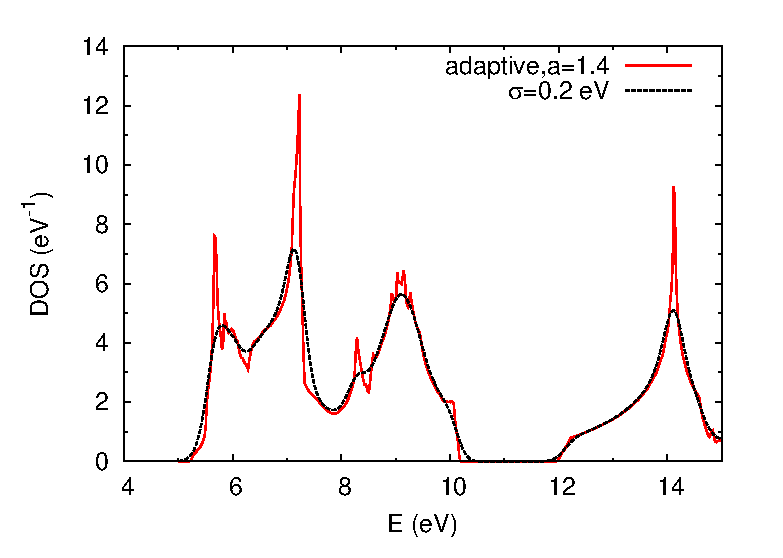
\includegraphics[width=0.45\textwidth]{DOS1-32.eps}
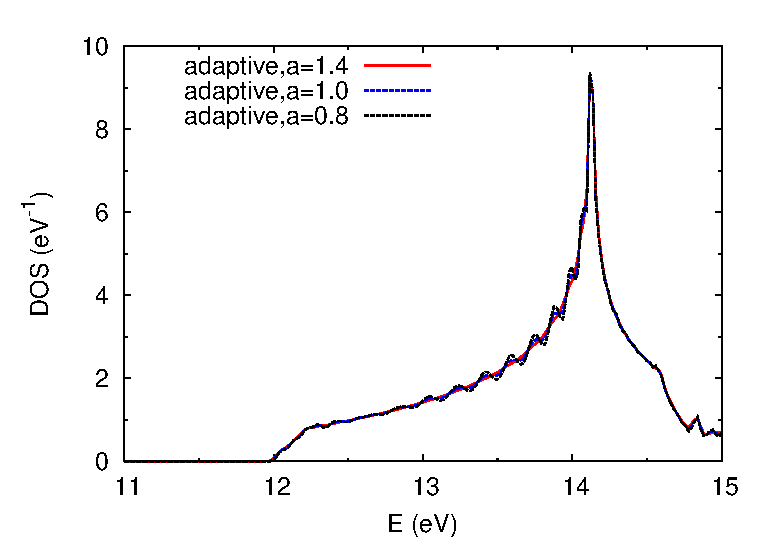
\includegraphics[width=0.45\textwidth]{DOS2-32.eps}
\caption{\label{fig:dos} Left: Comparison of constant smearing (width = 0.2eV) and adaptive smearing with $a=1.4$. 
Right: Comparison of different values of the parameter $a$. Fermi level corresponding to $n=10^{20} cm^{-3}$ is used.}
\end{figure}
%
%
\begin{figure}[!ht]
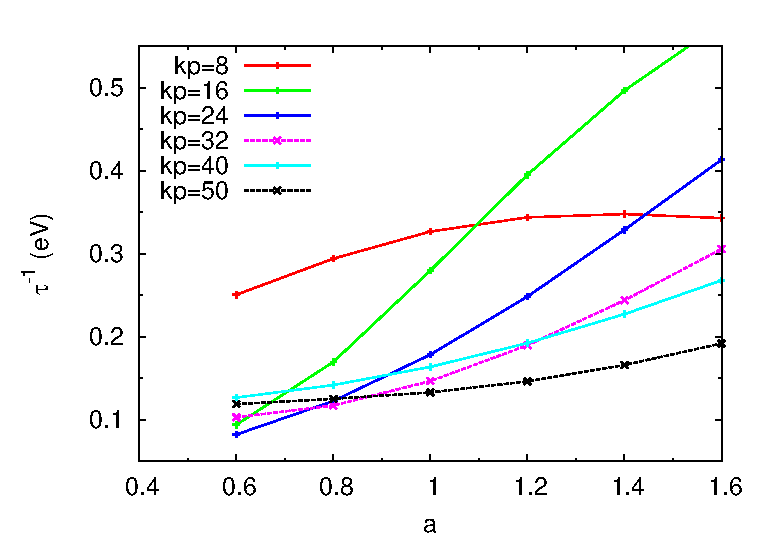
\includegraphics[width=0.45\textwidth]{invtau_vs_a.eps}
\caption{\label{fig:tauef} Calculated $D_n\, \tau^{-1}_n(E_F)$ for $c=10.0$ for different choices of k-point grid as a function of $a$.
Fermi level corresponding to $n=10^{20} cm^{-3}$ is used.}
\end{figure}
%
%
\begin{figure}[!ht]
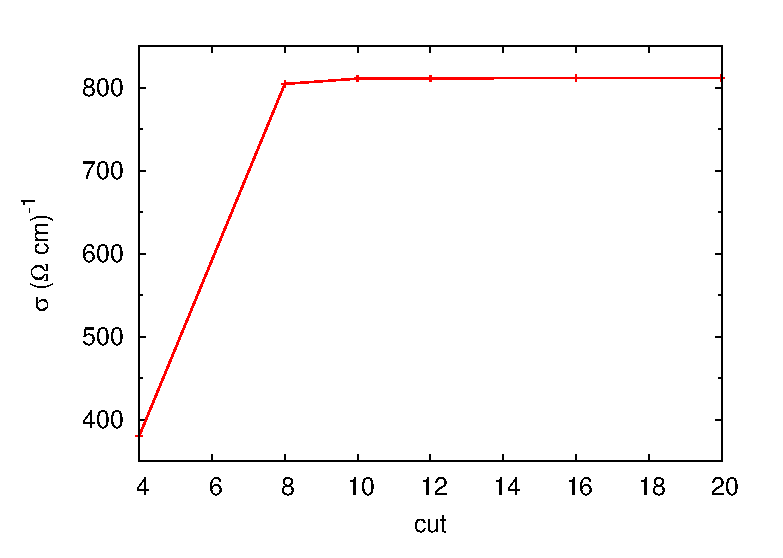
\includegraphics[width=0.45\textwidth]{sig_vs_cut.eps}
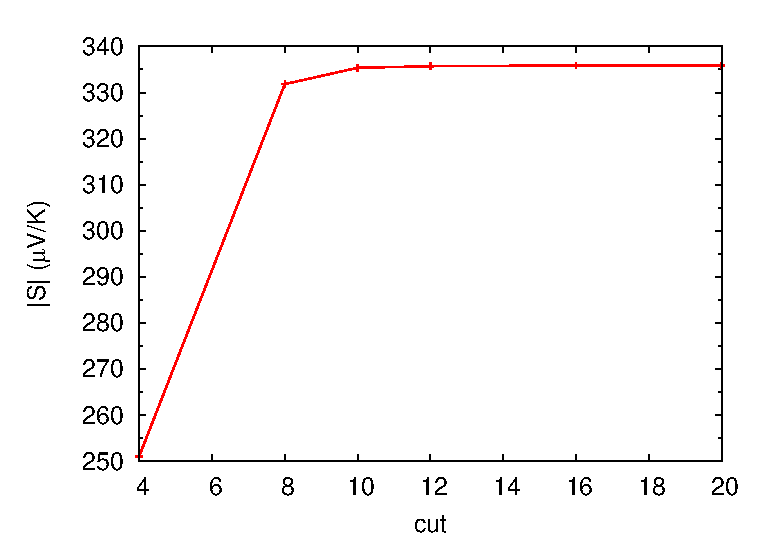
\includegraphics[width=0.45\textwidth]{Se_vs_cut.eps}
\caption{\label{fig:vs_cut} Calculated transport coefficients for $16 \times 16 \times 16$ grid with varying $c$,
using a constant scattering rate of 0.1 eV at 300 K.}
\end{figure}
%

%
\begin{figure}[!ht]
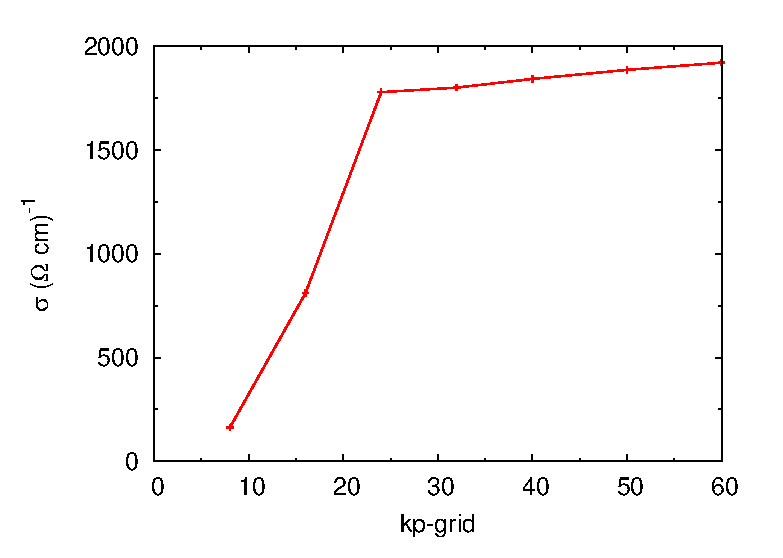
\includegraphics[width=0.45\textwidth]{sig_vs_kp.eps}
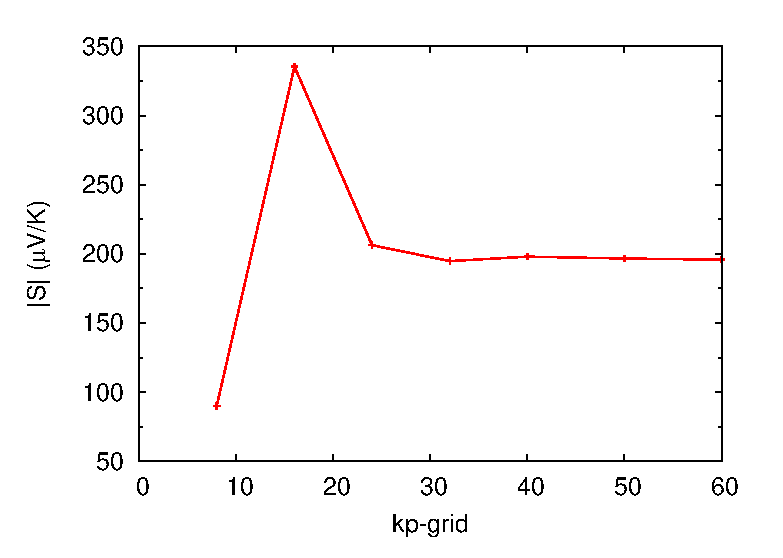
\includegraphics[width=0.45\textwidth]{Se_vs_kp.eps}
\caption{\label{fig:vs_kp} Calculated transport coefficients for $c=10.0$, with varying grids,
a constant scattering rate of 0.1 eV at 300 K.}
\end{figure}
%



%
%\begin{figure}[!ht]
%\includegraphics[width=0.40\textwidth]{ee-scattering.eps}
%\caption{\label{fig:ee} Schematic illustration of ee scattering. The corresponding decay rate of an electron into 2 electrons
%and a hole has the same probability.}
%\end{figure}
% 



\end{document}
